\documentclass[a4paper,20pt]{article}
\usepackage[utf8]{inputenc}
\usepackage{listings}
\usepackage{color}
\usepackage{graphicx}
\usepackage{verbatim}
\usepackage[margin=0.5in]{geometry}
\lstset{ %
  language=R,                     % the language of the code
  basicstyle=\footnotesize,       % the size of the fonts that are used for the code
  numbers=left,                   % where to put the line-numbers
  numberstyle=\tiny\color{gray},  % the style that is used for the line-numbers
  stepnumber=1,                   % the step between two line-numbers. If it's 1, each line
                                  % will be numbered
  numbersep=5pt,                  % how far the line-numbers are from the code
  backgroundcolor=\color{white},  % choose the background color. You must add \usepackage{color}
  showspaces=false,               % show spaces adding particular underscores
  showstringspaces=false,         % underline spaces within strings
  showtabs=false,                 % show tabs within strings adding particular underscores
  frame=single,                   % adds a frame around the code
  rulecolor=\color{black},        % if not set, the frame-color may be changed on line-breaks within not-black text (e.g. commens (green here))
  tabsize=2,                      % sets default tabsize to 2 spaces
  captionpos=b,                   % sets the caption-position to bottom
  breaklines=true,                % sets automatic line breaking
  breakatwhitespace=false,        % sets if automatic breaks should only happen at whitespace
  title=\lstname,                 % show the filename of files included with \lstinputlisting;
                                  % also try caption instead of title
  keywordstyle=\color{blue},      % keyword style
  commentstyle=\color{dkgreen},   % comment style
  stringstyle=\color{mauve},      % string literal style
  escapeinside={\%*}{*)},         % if you want to add a comment within your code
  morekeywords={*,...}            % if you want to add more keywords to the set
}
\definecolor{dkgreen}{rgb}{0,0.6,0}
\definecolor{gray}{rgb}{0.5,0.5,0.5}
\definecolor{mauve}{rgb}{0.58,0,0.82}
%opening
\title{Pattern Recognition and Data Mining HW4}
\author{Kevin Aloysius}

\begin{document}

\maketitle

\section*{Solution 4(a)}

\begin{lstlisting}[language=R]
transactions <- read.transactions(file = "ratingsAsBasket.txt")
summary(transactions)
\end{lstlisting}
\verbatiminput{summary_output.txt}
- The Number of baskets in the dataset is 10000
\newline
\newline
-From the Summary above the most frequent item rated high in the datasets is is the Movie 'The Matrix' with a freqency of 4729 in the movie ratings basket.
The Second most frequent movie in the basket is ``Pulp Fiction'' occuring 4610 times in the basket. Third highest rated movie in the basket is
``Saving Private Ryan'' with a frequency of 4162.  ``The Silence of the Lambs'' comes fourth
with a frequency of 4152 which is then followed by ``True Lies'' with an occurance of 4010 in the dataset.
\newline
\newline
From the Summary, the number of movies rated by a rater is as follows,\newline
The Minimum number of movies rated by one rater is 20.\newline
The Maximum number of movies rated by one rater is 2289.\newline
The Average number of movies rated by one rater is 153.6\newline
\newpage

\section*{Solution 4(b)}
\begin{lstlisting}[language=R]
transactions.apriori <- apriori(transactions)
inspect(transactions.apriori[1:10])
\end{lstlisting}
\begin{verbatim}
> inspect(transactions.apriori[1:10])

   lhs                rhs             support confidence     lift
1  {M.3816.R.High} => {M.3749.R.High}  0.1230  0.8698727 1.886926
2  {M.4033.R.High} => {M.4275.R.High}  0.1235  0.8178808 1.969848
3  {M.2175.R.High} => {M.2526.R.High}  0.1405  0.8126084 2.207575
4  {M.2181.R.High,                                               
    M.2434.R.High} => {M.3749.R.High}  0.1017  0.8168675 1.771947
5  {M.2181.R.High,                                               
    M.4275.R.High} => {M.3749.R.High}  0.1119  0.8021505 1.740023
6  {M.1740.R.High,                                               
    M.2526.R.High} => {M.1870.R.High}  0.1026  0.8009368 2.042164
7  {M.2175.R.High,                                               
    M.2936.R.High} => {M.2526.R.High}  0.1011  0.8700516 2.363628
8  {M.2175.R.High,                                               
    M.2749.R.High} => {M.2526.R.High}  0.1106  0.8475096 2.302390
9  {M.1870.R.High,                                               
    M.2175.R.High} => {M.2749.R.High}  0.1031  0.8029595 2.526619
10 {M.2175.R.High,                                               
    M.2250.R.High} => {M.2526.R.High}  0.1057  0.8649755 2.349838
\end{verbatim}
Let us consider the 1st association rule which is given by R as,
\begin{verbatim}
   lhs                rhs             support confidence     lift
1  {M.3816.R.High} => {M.3749.R.High}  0.1230  0.8698727 1.886926
\end{verbatim}
The association rule says that the movie raters who had ``Reservoir Dogs'' in their basket have a greater
chance of having the movie ``Pulp Fiction'' in the same basket. Support is the ratio of the number of times
two or more items occur to the total number of transactions. A Support of 0.1230 for the first association of says that ``Reservoir Dogs'' and ``Pulp Fiction''
were in the same basket for $12.3\%$ of the total transactions.
The Confidence which is given as  0.8698727
tells that the probablity of the movie ``Reservoir Dogs'' and ``Pulp Fiction'' appearing in the same basket
is 0.8698727
\newpage
\section*{Solution 4(c)}
\begin{lstlisting}[language = R]
transactions.subset <- subset(transactions.apriori, subset = lift > 3.0)
inspect(transactions.subset)
\end{lstlisting}
\begin{verbatim}
> inspect(transactions.subset)

   lhs                rhs            support confidence     lift
1  {M.1817.R.High,                                              
    M.647.R.High}  => {M.646.R.High}  0.1026  0.8234350 3.057687
2  {M.2936.R.High,                                              
    M.647.R.High}  => {M.646.R.High}  0.1164  0.8185654 3.039604
3  {M.2250.R.High,                                              
    M.2936.R.High,                                              
    M.647.R.High}  => {M.646.R.High}  0.1025  0.8464079 3.142993
4  {M.2250.R.High,                                              
    M.2749.R.High,                                              
    M.647.R.High}  => {M.646.R.High}  0.1006  0.8293487 3.079646
5  {M.2526.R.High,                                              
    M.2749.R.High,                                              
    M.647.R.High}  => {M.646.R.High}  0.1007  0.8440905 3.134387
6  {M.2250.R.High,                                              
    M.2526.R.High,                                              
    M.647.R.High}  => {M.646.R.High}  0.1158  0.8324946 3.091328
7  {M.2250.R.High,                                              
    M.5407.R.High,                                              
    M.647.R.High}  => {M.646.R.High}  0.1038  0.8166798 3.032602
8  {M.1870.R.High,                                              
    M.2250.R.High,                                              
    M.647.R.High}  => {M.646.R.High}  0.1084  0.8181132 3.037925
9  {M.2250.R.High,                                              
    M.4275.R.High,                                              
    M.647.R.High}  => {M.646.R.High}  0.1157  0.8390138 3.115536
10 {M.2250.R.High,                                              
    M.4712.R.High,                                              
    M.647.R.High}  => {M.646.R.High}  0.1130  0.8242159 3.060586
11 {M.2526.R.High,                                              
    M.5407.R.High,                                              
    M.647.R.High}  => {M.646.R.High}  0.1012  0.8214286 3.050236
12 {M.1870.R.High,                                              
    M.2526.R.High,                                              
    M.647.R.High}  => {M.646.R.High}  0.1072  0.8195719 3.043341
13 {M.2526.R.High,                                              
    M.4275.R.High,                                              
    M.647.R.High}  => {M.646.R.High}  0.1119  0.8369484 3.107866
14 {M.2526.R.High,                                              
    M.4712.R.High,                                              
    M.647.R.High}  => {M.646.R.High}  0.1075  0.8231240 3.056532
15 {M.4275.R.High,                                              
    M.5407.R.High,                                              
    M.647.R.High}  => {M.646.R.High}  0.1066  0.8149847 3.026308
16 {M.1870.R.High,                                              
    M.4275.R.High,                                              
    M.647.R.High}  => {M.646.R.High}  0.1085  0.8238421 3.059198
17 {M.4275.R.High,                                              
    M.4712.R.High,                                              
    M.647.R.High}  => {M.646.R.High}  0.1112  0.8261516 3.067774
\end{verbatim}

Let us consider the 1st in the above rule where the lift is greater than 3.0
The association rule states that,
\begin{verbatim}
   lhs                rhs            support confidence     lift
1  {M.1817.R.High,                                              
    M.647.R.High}  => {M.646.R.High}  0.1026  0.8234350 3.057687
\end{verbatim}

Lift indicates the strength of an association rule over the random
occurance co-occurance of the movie\newline``Aliens'',``Terminator 2: Judgment Day'' and the movie ``The Terminator''. Lift provides information about the change in the
probablity of Item A in the presence of Item B. Lift values greater than 3.0 indicate that transactions
containing ``The Terminator'' has ``Aliens'' and ``Terminator 2: Judgment Day'' more often than transactions
that do not contain ``The Terminator''.
\newpage
\section*{Solultion 5(a)}
\begin{lstlisting}[language = R]
directory <- c("/home/kevin/DataMining/DataMiningHW4/rec.motorcycles","/home/kevin/DataMining/DataMiningHW4/rec.autos")
dir_source <- DirSource(directory = directory, encoding = "UTF-8")
news.corpus <- VCorpus(dir_source, readerControl = list(reader = reader(dir_source)))
\end{lstlisting}
\begin{verbatim}
> news.corpus
> <<VCorpus (documents: 1986, metadata (corpus/indexed): 0/0)>>

> length(news.corpus)
[1] 1986

> news.corpus[[980]]
<<PlainTextDocument (metadata: 7)>>
From: cheekeen@tartarus.uwa.edu.au (Desmond Chan)
Subject: Re: Honda clutch chatter
Organization: The University of Western Australia
Lines: 8
NNTP-Posting-Host: tartarus.uwa.edu.au
X-Newsreader: NN version 6.4.19 #1

     I also experience this kinda problem in my 89 BMW 318. During cold
start ups, the clutch seems to be sticky and everytime i drive out, for
about 5km, the clutch seems to stick onto somewhere that if i depress
the clutch, the whole chassis moves along. But after preheating, it
becomes smooth again. I think that your suggestion of being some
humudity is right but there should be some remedy. I also found out that
my clutch is already thin but still alright for a couple grand more!
\end{verbatim}
\newpage
\section*{Solution 5(b)}
\begin{lstlisting}[language = R]
# Applying the removePunctuation over the news.corpus
news.corpus <- tm_map(news.corpus, removePunctuation)
news.corpus <- VCorpus(VectorSource(news.corpus))
\end{lstlisting}
\begin{verbatim}
> news.corpus[[980]]
<<PlainTextDocument (metadata: 7)>>
From cheekeentartarusuwaeduau Desmond Chan
Subject Re Honda clutch chatter
Organization The University of Western Australia
Lines 8
NNTPPostingHost tartarusuwaeduau
XNewsreader NN version 6419 1

     I also experience this kinda problem in my 89 BMW 318 During cold
start ups the clutch seems to be sticky and everytime i drive out for
about 5km the clutch seems to stick onto somewhere that if i depress
the clutch the whole chassis moves along But after preheating it
becomes smooth again I think that your suggestion of being some
humudity is right but there should be some remedy I also found out that
my clutch is already thin but still alright for a couple grand more
\end{verbatim}

\begin{lstlisting}[language = R]
# Applying removeNumbers over news.corpus
news.corpus <- tm_map(news.corpus, removeNumbers)
news.corpus <- VCorpus(VectorSource(news.corpus))
\end{lstlisting}
\begin{verbatim}
> news.corpus[980]
<<PlainTextDocument (metadata: 7)>>
From cheekeentartarusuwaeduau Desmond Chan
Subject Re Honda clutch chatter
Organization The University of Western Australia
Lines 
NNTPPostingHost tartarusuwaeduau
XNewsreader NN version  

     I also experience this kinda problem in my  BMW  During cold
start ups the clutch seems to be sticky and everytime i drive out for
about km the clutch seems to stick onto somewhere that if i depress
the clutch the whole chassis moves along But after preheating it
becomes smooth again I think that your suggestion of being some
humudity is right but there should be some remedy I also found out that
my clutch is already thin but still alright for a couple grand more
\end{verbatim}

\begin{lstlisting}[language = R]
# Applying tolower to news.corpus
news.corpus <- tm_map(news.corpus, tolower)
news.corpus <- VCorpus(VectorSource(news.corpus))
\end{lstlisting}
\begin{verbatim}
> news.corpus[[980]]
<<PlainTextDocument (metadata: 7)>>
from cheekeentartarusuwaeduau desmond chan
subject re honda clutch chatter
organization the university of western australia
lines 
nntppostinghost tartarusuwaeduau
xnewsreader nn version  

     i also experience this kinda problem in my  bmw  during cold
start ups the clutch seems to be sticky and everytime i drive out for
about km the clutch seems to stick onto somewhere that if i depress
the clutch the whole chassis moves along but after preheating it
becomes smooth again i think that your suggestion of being some
humudity is right but there should be some remedy i also found out that
my clutch is already thin but still alright for a couple grand more
\end{verbatim}

\begin{lstlisting}[language = R]
# Applying removeWords stopwords("english")
news.corpus <- tm_map(news.corpus, removeWords, stopwords("english"))
news.corpus <- VCorpus(VectorSource(news.corpus))
\end{lstlisting}
\begin{verbatim}
> news.corpus[[980]]
<<PlainTextDocument (metadata: 7)>>
 cheekeentartarusuwaeduau desmond chan
subject re honda clutch chatter
organization  university  western australia
lines 
nntppostinghost tartarusuwaeduau
xnewsreader nn version  

      also experience  kinda problem    bmw   cold
start ups  clutch seems   sticky  everytime  drive  
 km  clutch seems  stick onto somewhere    depress
 clutch  whole chassis moves along   preheating 
becomes smooth   think   suggestion   
humudity  right      remedy  also found  
 clutch  already thin  still alright   couple grand
\end{verbatim}

\section*{Solution 5(c)}
\begin{lstlisting}[language = R]
dtm <- DocumentTermMatrix(news.corpus, control = list(minWordLength = 1, minDocFreq = 1))
\end{lstlisting}
\begin{verbatim}
> dim(dtm)
[1]  1986 22213

> dtm
<<DocumentTermMatrix (documents: 1986, terms: 22213)>>
Non-/sparse entries: 175981/43939037
Sparsity           : 100%
Maximal term length: 163
Weighting          : term frequency (tf)

> inspect(news.corpus[[980]])
<<VCorpus (documents: 1, metadata (corpus/indexed): 0/0)>>

[[1]]
<<PlainTextDocument (metadata: 7)>>
 cheekeentartarusuwaeduau desmond chan
subject re honda clutch chatter
organization  university  western australia
lines 
nntppostinghost tartarusuwaeduau
xnewsreader nn version  

      also experience  kinda problem    bmw   cold
start ups  clutch seems   sticky  everytime  drive  
 km  clutch seems  stick onto somewhere    depress
 clutch  whole chassis moves along   preheating 
becomes smooth   think   suggestion   
humudity  right      remedy  also found  
 clutch  already thin  still alright   couple grand
\end{verbatim}

\section*{Solution 2 (a)}
\begin{lstlisting}[language = R]
# Solution(5)
# Kevin Aloysius
# Reading az-5000.txt data
set.seed(1)
char <- read.table("az-5000.txt", header = TRUE)
# Removing the first Column
char <- char[,2:19]
# Applying kmeans() to calculate the number of clusters
fit <- vector()

for (i in 2:26)
{
  output <- kmeans(char, centers = i, iter.max = 26)
  fit[i] <- (1/i)*sum(kmeans(char, centers = i)$withinss)
}
plot(1:26, fit, type = "b", xlab = "Number of Clusters", ylab = "Goodness of Fit (withinss)",
     main = "Number of Clusters v/s Goodness of Fit")

# Applying kmeans from 15 to 26 to calculate the number of clusters
fit2 <- vector()

for (i in 15:26)
{
  
  fit2[i] <- (1/i)*sum(kmeans(char, centers = i)$withinss)
}
plot(1:26, fit2, type = "b", xlab = "Number of Clusters", ylab = "Goodness of Fit (withinss)",
     main = "Number of Clusters v/s Goodness of Fit")


\end{lstlisting}
\section*{Solution 2 (b)}
\begin{center}
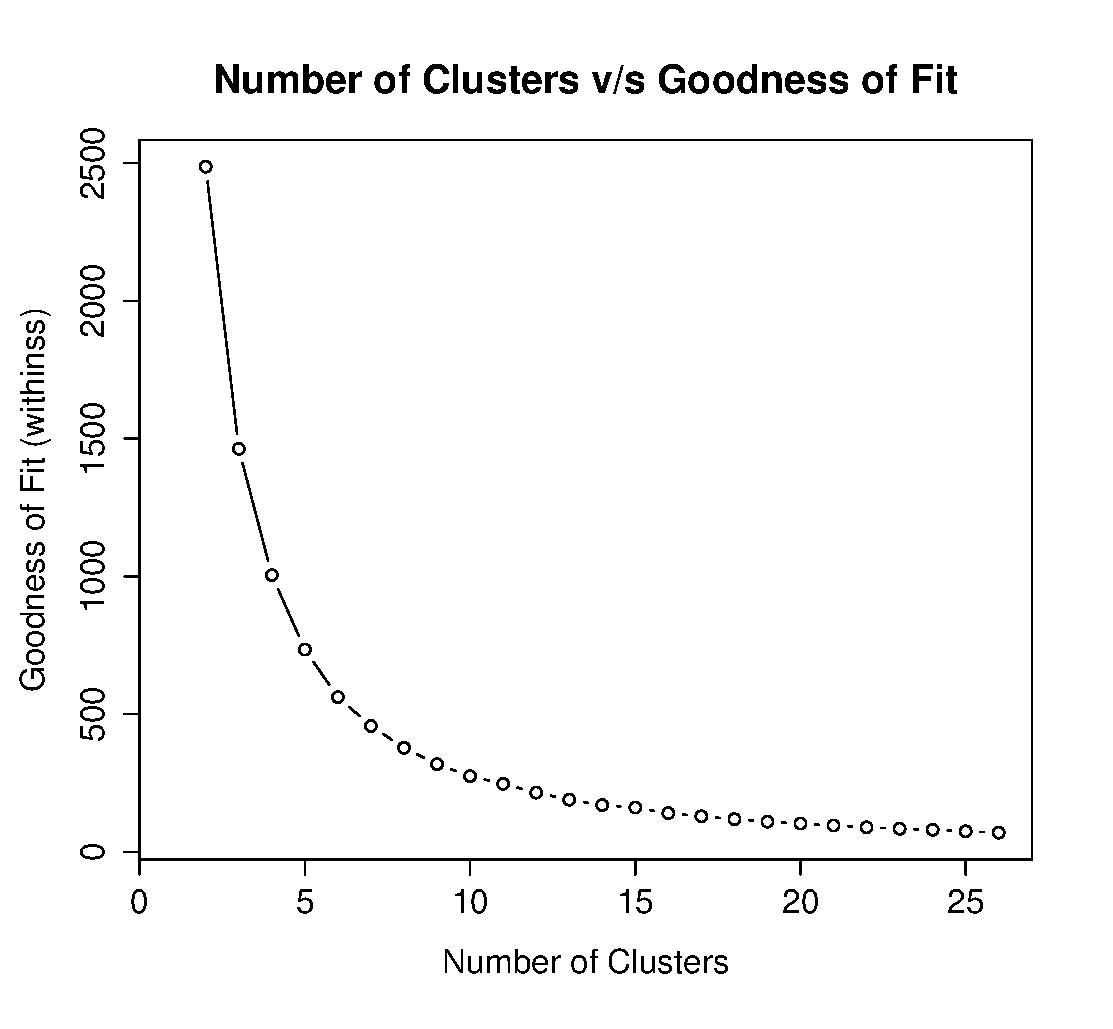
\includegraphics[scale=0.7]{cluster_goodness.eps}
\end{center}
\begin{center}
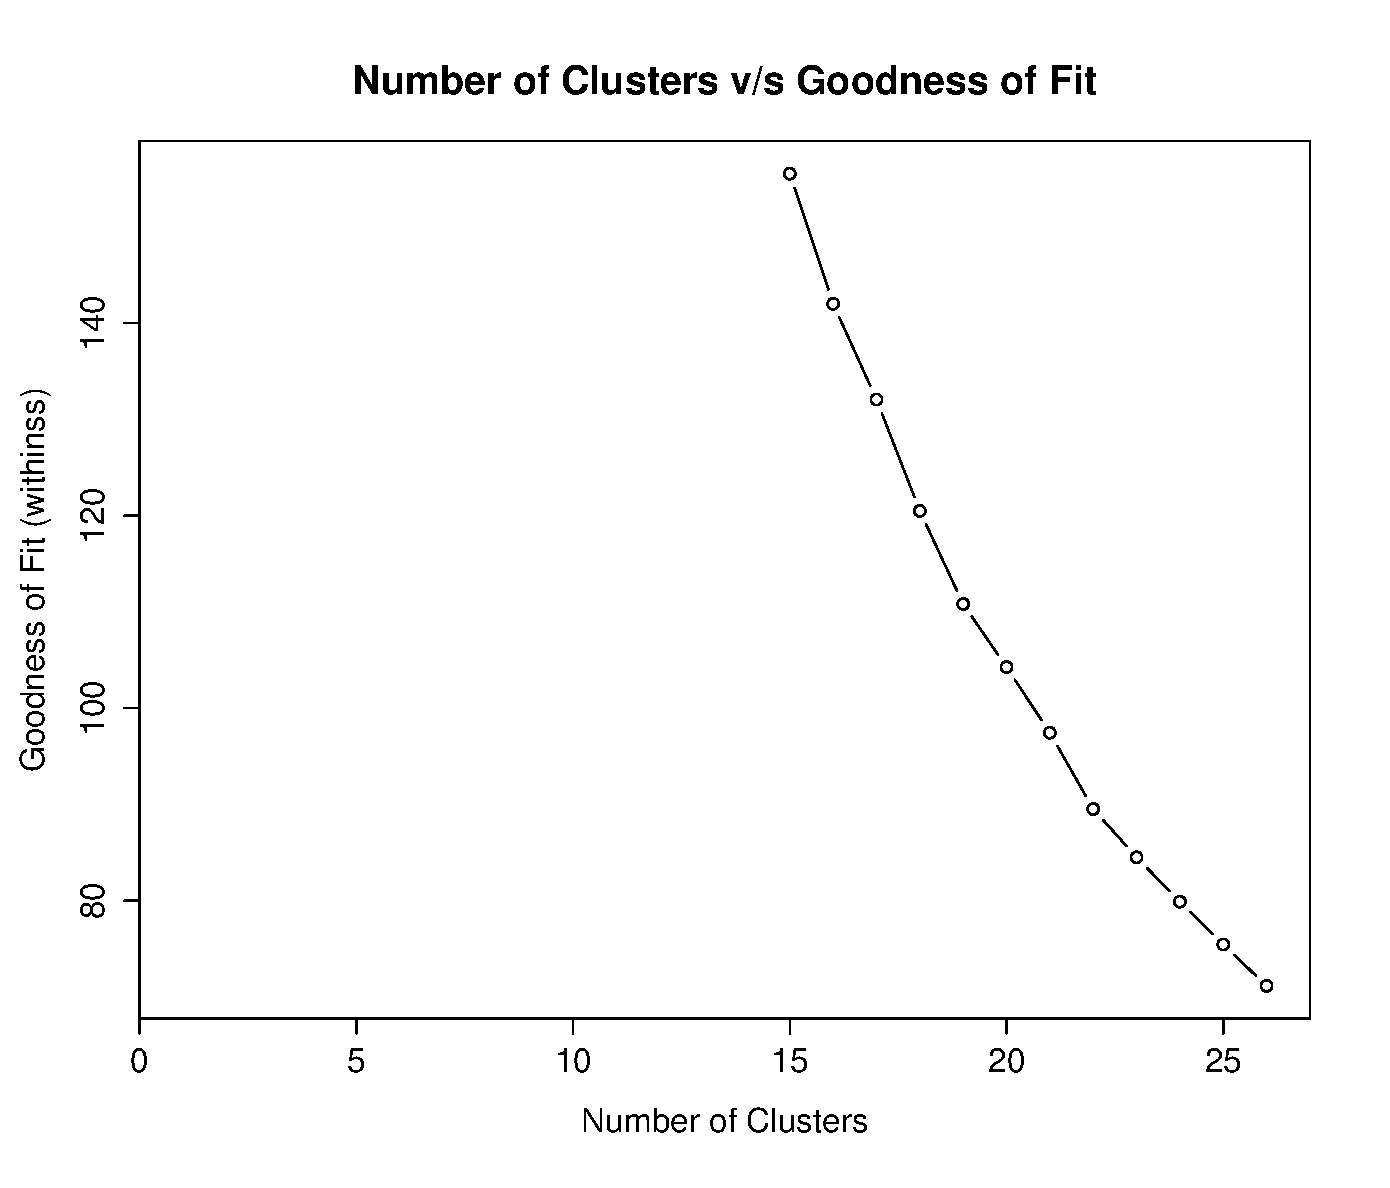
\includegraphics[scale=0.7]{kmeans_cluster.eps}
\end{center}
The 23rd letter 'W' suggests the number of natural clusters. This is because
after plotting the number of K's from 15 to 26, we could observe a dip at 23 suggesting
the number of clusters.
\newpage
\section*{Solution 3 (a)}
\begin{lstlisting}[language = R]
# Hierarchial Clustering
# Kevin Aloysius
set.seed(123)

# Loading the data
character <- read.table("az-5000.txt", header = TRUE)

# Removing the first column
char <- character[,-1]

# Applying kmeans
fit <- vector()
for (i in 2:26)
{
  output <- kmeans(char, centers = i, iter.max = 26)
  
}

# Hierarchial Clustering
fit <- hclust(a <- dist(output$centers, method = "euclidean"), method="average")
plot(fit)
\end{lstlisting}
\begin{center}
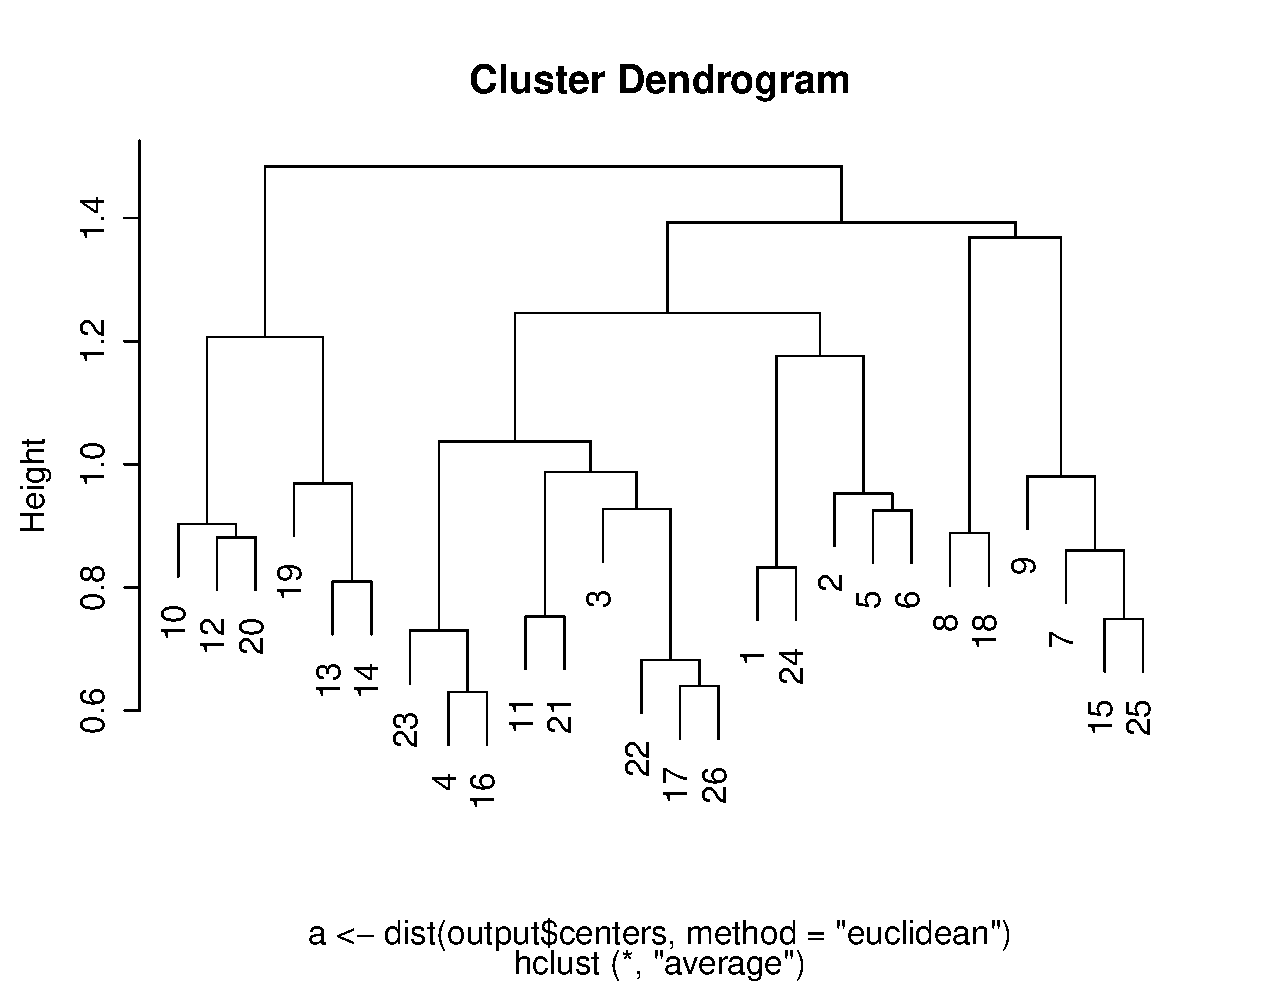
\includegraphics[scale=0.7]{dendogram.eps}
\end{center}
\newpage
\section*{Solution 3 (b)}
\begin{lstlisting}[language = R]
# 26x26 Matrix Mapping, Letters vs Cluster numbers

letter_matrixrix <- character[,1]
num_cluster <- output$cluster 
matrix <- matrix(0,26,26)
rownames(matrix) <- LETTERS

for(k in 1:5000)
{ 
  matrix[letter_matrix[k], num_cluster[k]] <-  matrix[letter_matrix[k], num_cluster[k]] + 1
}

# Replacing Values of Dendograms with Letters
common <- c()
for(i in 1:26)
{
  common[i] <- which.max(matrix[,i])
}

plot(fit, labels=LETTERS[common])
\end{lstlisting}
\begin{center}
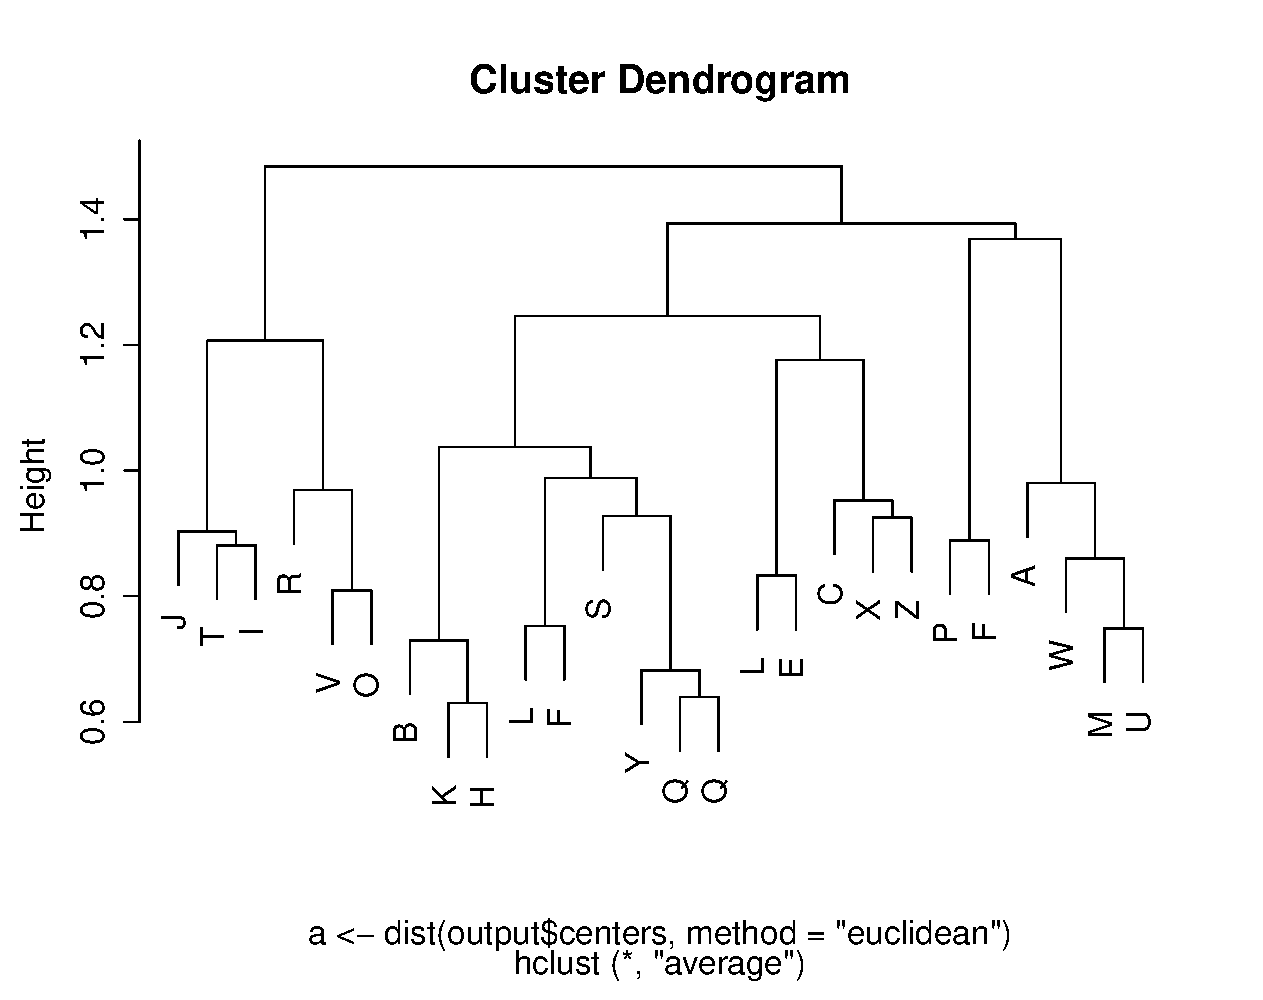
\includegraphics[scale=0.7]{dendogram_letters.eps}
\end{center}
\newpage
\section*{Solution 6}
\begin{lstlisting}[language = R]
# Kevin Aloysius
set.seed(123)
#using the letter confusion matrix from HW2 for this question

Chars <- read.table("az-5000.txt", header = TRUE) 
dim(Chars) 

train <- sample(1:5000, 4000) 

table(Chars$char[train]) 

char.priors <- c(rep(1/26, 26)) 

Char.lda <- lda(char ~., Chars, subset = train, prior = char.priors) 

Char.confusion <- table(Chars[-train, ]$char, predict(Char.lda, Chars[-train, ])$class)

#setting diagonals of the matrix to be 0 and producing image with non-zero entries colored
diag(Char.confusion) <- 0
labelpos <- 0:25
labelpos_std <- labelpos/25
image(Char.confusion, col=heat.colors(4), axes=FALSE)
axis(1, labelpos_std, labels=LETTERS[1:26])
axis(2, labelpos_std, labels=LETTERS[1:26])
\end{lstlisting}
\section*{Solution 6(a)}
\begin{center}
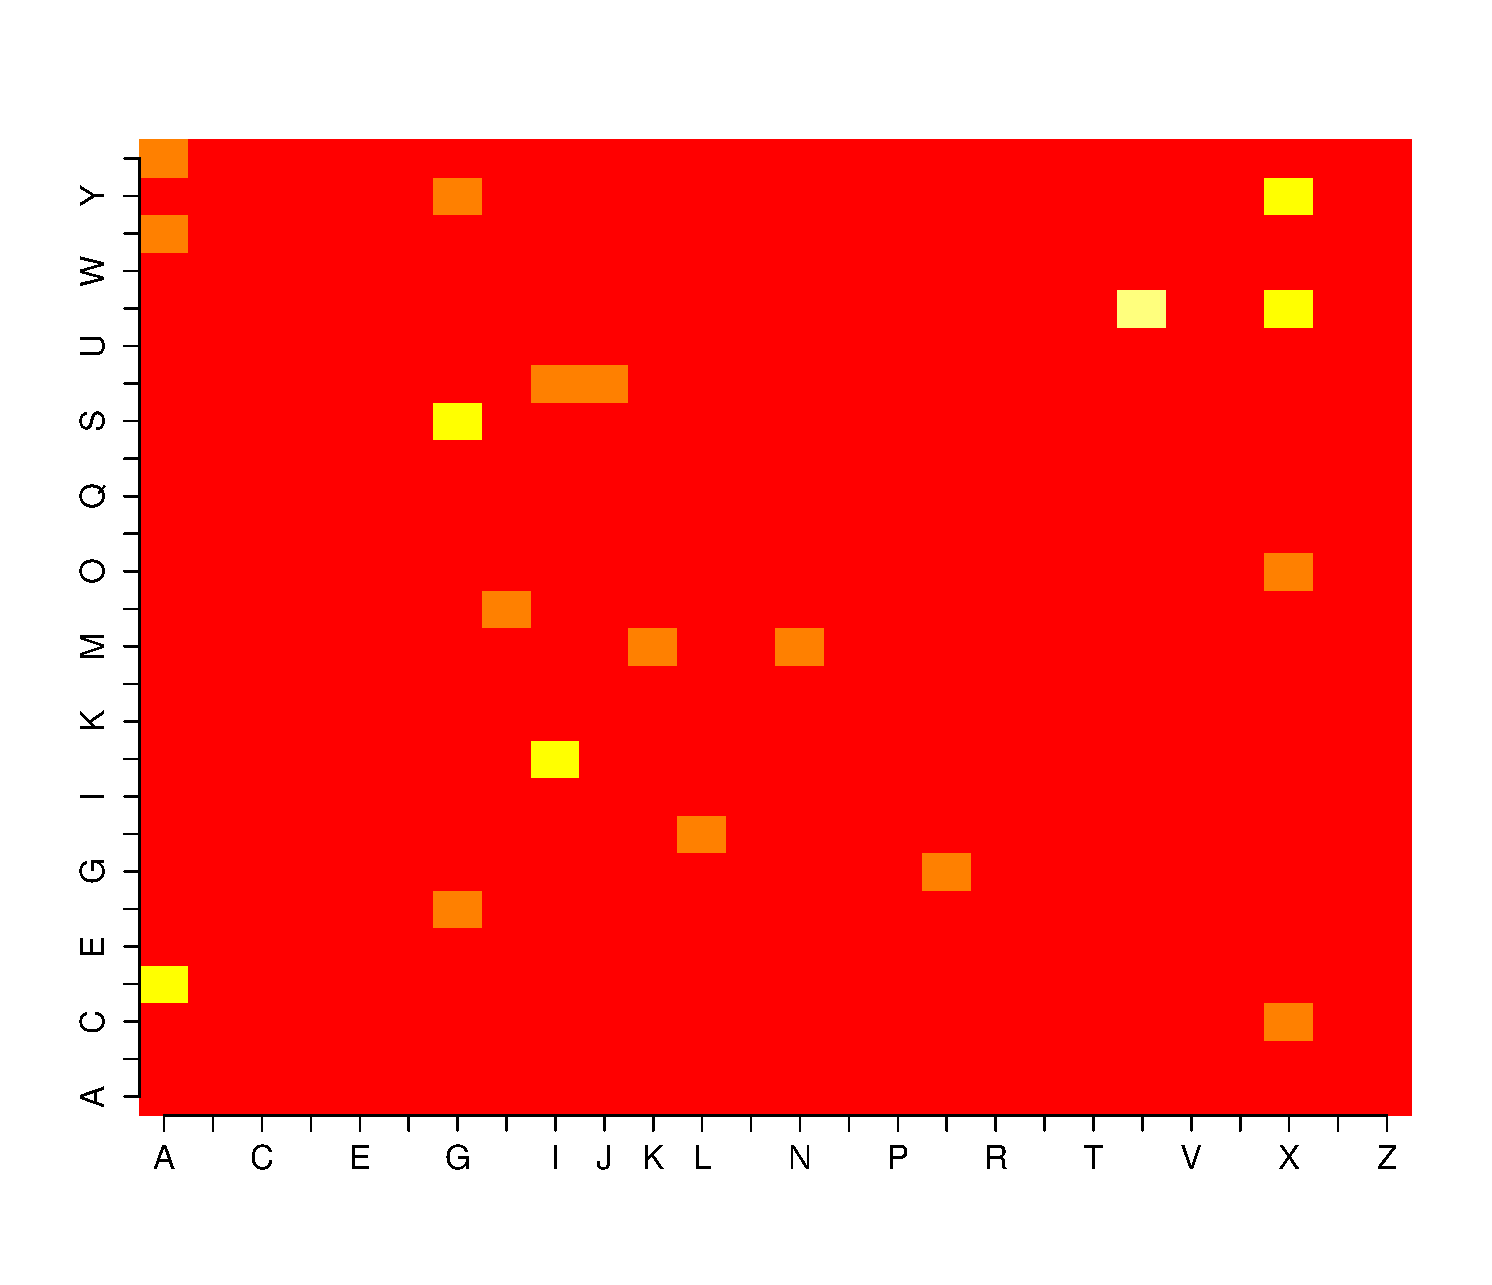
\includegraphics[scale=0.7]{visuals.eps}
\end{center}
\section*{Solution 6(b)}
The Letter pair with the worst confusion matrix from the above diagram is the Letter Pair {V,U} (Row 'V' and Column 'U'). It is represented in white color and the value of this matrix is 8.
\end{document}